\documentclass[11pt,a4paper]{article}
\usepackage[margin=25mm]{geometry}
\usepackage[T1]{fontenc}
\usepackage{lmodern}
\usepackage{amsmath,amssymb,booktabs,array,graphicx}
\usepackage[numbers,sort&compress]{natbib}
\usepackage{microtype}
\usepackage{url}
\usepackage[hidelinks]{hyperref}
\usepackage[font=small,labelfont=bf]{caption}
\usepackage{enumitem}
\usepackage{listings}
\usepackage{placeins}
\hypersetup{pdftitle={video2xy: Converting Raster Video to Stereo XY Oscilloscope Signals},pdfauthor={Peter Schwendner}}
\lstset{basicstyle=\ttfamily\small,breaklines=true,columns=fullflexible,keepspaces=true}
\setlength{\parskip}{3pt}
\setlength{\emergencystretch}{2em}
\newcommand{\code}[1]{\texttt{#1}}
\newcommand{\R}{\mathbb{R}}
\title{\textbf{video2xy: Converting Raster Video to\newline Stereo XY Oscilloscope Signals}}
\author{Peter Schwendner\\[3pt]
\small Zurich University of Applied Sciences\\
\small\href{mailto:scwp@zhaw.ch}{\texttt{scwp@zhaw.ch}}}
\date{September 13, 2026}
\begin{document}
\maketitle
\begin{abstract}
An oscilloscope in XY mode can display a two-dimensional trajectory driven by stereo audio. Inspired by oscilloscope music, \emph{video2xy} converts raster video or camera frames into such signals through edge selection, contour simplification, adjacent-frame association, and arc-length resampling under a fixed scan budget. This paper describes a revised implementation with vectorized resampling, explicit budget and timing validation, and a shared scan scheduler for WAV export and live output. At 44.1~kHz and 60 scans/s, each drawing contains 735 stereo sample pairs. All 29 regression tests pass. The revised resampler matches the original exactly in 3,000 random and 300 structured cases, and tracking retains exact waveform invariance in 200 trials of a restricted three-rectangle representation test. A 25~frames/s export test verifies continuous scan phase across video-frame boundaries. In an interleaved fixed-image benchmark, mean processing time decreases from 26.89 to 19.07~ms per frame; decoding and output devices are excluded. Frame-clock checks over 100,000 frames at each of four video rates stay within half a sample of ideal elapsed time. These results establish finite software checks, not analog display fidelity, sustained real-time performance, or general perceptual improvement. AI assistance in implementation, review, and manuscript preparation is disclosed.

\end{abstract}
\noindent\textbf{Keywords:} XY oscilloscope; vector display; raster vectorization; contour tracking; audio signal synthesis; digital-to-analog conversion.

\section{Introduction}
In an XY display, horizontal and vertical deflection are controlled by separate signals rather than by a horizontal time base. A stereo digital audio stream can therefore encode a planar trajectory: its left channel supplies the horizontal coordinate, and its right channel supplies the vertical coordinate. Oscilloscope Music, developed by Jerobeam Fenderson and Hansi Raber, demonstrates an artistic use of this correspondence in which the same signals generate both sound and visual form~\cite{oscimusic}. The display is an interpretation of the signal itself, rather than a visualization computed from an unrelated soundtrack.

The project considered here, \emph{video2xy}~\cite{video2xy}, starts from raster images. It selects image contours and schedules their traversal as a periodic stereo signal. This changes the engineering problem: extracted boundaries must fit into a finite sample budget, disconnected curves require visible repositioning, and frame-to-frame changes in contour representation can alter the waveform even when the depicted geometry does not change. The sound is a consequence of the selected paths and their timing; the program does not preserve the input video's soundtrack or optimize musical composition.

The contribution is a documented integration of established image-processing operations with lightweight temporal scan stabilization and a shared scan scheduler with distinct file and live timing. It is not a claim to have invented sound-driven vector graphics, raster tracing, or contour association. The analysis distinguishes what the program implements, what follows analytically under stated assumptions, and what has been checked by executing software. The revised implementation is local commit \code{cc7fe7a82c60}, based on the public September 11, 2026 revision \code{6a7d1dd8be76}. The source package includes both the update and the original module used for comparisons. Full identifiers and publication status are given in Section~\ref{sec:repro}.

\section{Related work}
OsciStudio converts three-dimensional shapes and animations into sound and provides parameter animation and sound modification~\cite{oscistudio}. Holzer's Vector Synthesis library explores the direct relation between sound and vector imagery using Pure Data, including multiplexing, coordinate transformations, and a separate intensity signal for blanking~\cite{holzer}. These systems establish both the audiovisual context and the practical significance of phase, bandwidth, and beam repositioning. The present two-channel design has no independent intensity output.

Other software substantially overlaps the broader application space. In particular, osci-render supports objects, vector images, text, Blender integration, and programmable synthesis~\cite{oscirender}; its documented releases also include PNG, JPEG, and animated-GIF input~\cite{oscirenderimages}. Accordingly, raster-to-oscilloscope conversion is not presented as a novel application category. The narrower purpose of video2xy is to expose a short, inspectable path from video frames to contour-based audio, with explicit adjacent-frame scan stabilization and file or camera input.

The processing stages use CLAHE for contrast enhancement~\cite{zuiderveld}, Canny edge detection~\cite{canny}, border-following contour extraction~\cite{suzuki}, and Douglas--Peucker polygon simplification~\cite{douglas}. OpenCV supplies the corresponding implementation primitives~\cite{opencvshape,opencvfilter}. The temporal matcher and sample scheduler described below are project-specific combinations of geometric heuristics. They have no learned parameters and require no model training.

\section{System model and processing pipeline}
Let $I_k$ denote video frame $k$, $f_v$ the nominal frame rate, $f_s$ the stereo sample rate, and $f_r$ the requested retrace rate. The program produces a scan
\begin{equation}
 S_k[n]=\bigl(x_k[n],y_k[n]\bigr),\qquad 0\leq n<N,
 \quad N=\max\!\left(16,\operatorname{round}(f_s/f_r)\right).
 \label{eq:scan}
\end{equation}
Here a ``sample'' means one simultaneous XY pair, not one scalar channel value. The actual repetition frequency is $\widehat f_r=f_s/N$. At the defaults, $f_s=44{,}100$~Hz and $f_r=60$~Hz give $N=735$ and $\widehat f_r=60$~Hz exactly. Other settings need not realize the requested frequency exactly; the lower bound on $N$ also limits the maximum repetition rate.

The processing chain is
\begin{center}
\small
video frame $\longrightarrow$ selected edges $\longrightarrow$ simplified contours\\[3pt]
$\longrightarrow$ temporally ordered paths $\longrightarrow$ sampled XY scan\\[3pt]
$\longrightarrow$ WAV export or live stereo output $\longrightarrow$ XY display.
\end{center}
Table~\ref{tab:defaults} specifies the principal defaults. Input is opened with \code{cv2.VideoCapture}; a purely numeric input string is interpreted as a camera index. An explicit \code{--fps} overrides reported frame rate, and automatic timing falls back to 30~frames/s for unavailable, nonfinite, or at most 0.001~frames/s metadata. Other resolved rates must be positive and no greater than the audio sample rate. The implementation uses nominal frame timing rather than presentation timestamps, so variable-frame-rate sources are not reproduced with their original timing.

\begin{table}[t]
\centering\small
\caption{Principal defaults in the inspected implementation. Pixel quantities refer to the resized image.}
\label{tab:defaults}
\begin{tabular}{@{}>{\raggedright\arraybackslash}p{.39\linewidth}>{\raggedright\arraybackslash}p{.21\linewidth}>{\raggedright\arraybackslash}p{.33\linewidth}@{}}
\toprule
Control & Default & Role\\\midrule
Audio and retrace rates & 44,100 Hz; 60 Hz & 735 XY samples per scan\\
Processing width & 480 pixels & Proportional height scaling\\
CLAHE & 1.5; $8\times8$ tiles & Local contrast enhancement\\
Gaussian and Sobel kernels & $5\times5$; $3\times3$ & Smoothing and gradients\\
Sobel percentile & 72 & Threshold over positive magnitudes\\
Canny thresholds & 35; 110 & Hysteresis thresholds\\
Morphological closing & One $3\times3$ iteration & Edge-gap connection\\
Contour limits & 18 pixels; 32 contours & Minimum perimeter; maximum count\\
Simplification fraction & 0.004 & Tolerance relative to perimeter\\
Tracking distance & 0.08 & Fraction of image diagonal\\
Samples per contour and jump & 8; 1 & Minimum allocation; repositioning\\
Scope aspect and amplitude & 1.25; 0.80 & Display mapping and digital scale\\\bottomrule
\end{tabular}
\end{table}

\subsection{Edge selection}
Frames are resized proportionally with OpenCV's area interpolation and converted from BGR to grayscale. Optional contrast-limited adaptive histogram equalization (CLAHE) uses an $8\times8$ tile grid; a zero clip setting disables it. The CLI creates the configured CLAHE object once and reuses it across frames; negative clip settings are rejected. Gaussian smoothing precedes both Sobel gradients and Canny detection. For the smoothed image $G_k$, the program computes
\begin{equation}
 M_k(u,v)=\sqrt{G_{x,k}(u,v)^2+G_{y,k}(u,v)^2},\qquad
 \tau_k=Q_p\!\left(\{M_k(u,v):M_k(u,v)>0\}\right),
 \label{eq:edge}
\end{equation}
where $Q_p$ is the selected percentile. Canny is applied to the smoothed grayscale image with its Euclidean-gradient option enabled. The binary result is intersected with $[M_k\geq\tau_k]$, then morphologically closed if requested. If there are no positive gradient magnitudes, the Sobel mask is zero.

This is an intersection of two edge-selection mechanisms: Canny supplies thin candidate edges and the percentile gate rejects weak gradient locations. Raising the percentile can remove useful low-contrast boundaries as well as texture. Closing can repair gaps, but can also join nearby features. These are deliberate controls over drawing complexity, not a semantic foreground detector.

\subsection{Contour extraction and simplification}
\code{findContours} uses \code{RETR\_LIST} and \code{CHAIN\_APPROX\_NONE}. Thus, contour hierarchy is not retained and the initial chains include all boundary points. Each chain has a closed perimeter $P_i$; chains shorter than the configured minimum are discarded. Polygon simplification uses tolerance $\epsilon_i=\max(0,\epsilon_{\rm frac})P_i$ with closure enabled. Polygons with fewer than three vertices are discarded, and survivors are ranked by their original perimeters before the count limit is applied.

This representation follows boundaries in an edge image, not a skeleton of its strokes. A single apparent object can yield multiple contours, including close inner and outer boundaries. Moreover, all accepted paths are treated as closed, even when the source scene suggests an open stroke. Simplification and contour selection therefore define a lossy geometric abstraction of the input.

\section{Temporal contour association and scan stabilization}
\subsection{Adjacent-frame association}
Contour identity is estimated from bounding-box center $\mathbf c_i$, bounding-box extent $\mathbf e_i$, and simplified perimeter $L_i$. Each extent component is clamped to a minimum of one pixel. With tracking-distance fraction $\delta$ (default 0.08), an old contour $i$ and a new contour $j$ define
\begin{align}
 d_{ij}&=\|\mathbf c_j-\mathbf c_i\|_2, &
 s_{ij}&=\|\log(\mathbf e_j/\mathbf e_i)\|_\infty,\\
 \ell_{ij}&=\left|\log\frac{\max(L_j,10^{-6})}{\max(L_i,10^{-6})}\right|, &
 D&=\delta\sqrt{W^2+H^2}.
\end{align}
Logarithms and division of extent vectors act componentwise. A candidate must satisfy $d_{ij}\leq D$, $s_{ij}\leq\log2$, and $\ell_{ij}\leq\log2$. Its cost is
\begin{equation}
 a_{ij}=\frac{d_{ij}}{\max(D,10^{-6})}+s_{ij}+\ell_{ij}.
 \label{eq:association}
\end{equation}
All admissible pairs are sorted by cost. The algorithm accepts a pair if neither member has already been assigned. This is a greedy one-to-one assignment over the candidate set; it does not minimize total assignment cost globally.

Matched contours retain the previous scan order. Unmatched old contours disappear immediately, while new contours are appended after surviving tracks using nearest-start ordering. When no tracks survive, ordering starts with the first supplied contour, normally the longest retained contour. An empty detection set or change of frame dimensions clears tracking state. There is no motion prediction, occlusion memory, or persistence of old geometry. For up to $M$ old and $M$ new contours, candidate construction is $O(M^2)$ and sorting is $O(M^2\log M)$, apart from contour-description and alignment work.

\subsection{Starting point and traversal direction}
Retaining identity and order is insufficient: rotating a closed contour's vertex list or reversing its direction leaves its geometry unchanged but alters its coordinate waveforms. For each match, the old starting point $\mathbf p_{i,0}$ is translated by the bounding-box-center displacement,
\begin{equation}
 \mathbf t=\mathbf p_{i,0}+\mathbf c_j-\mathbf c_i.
\end{equation}
The nearest projection of $\mathbf t$ onto any segment of the new polygon becomes the new starting point. Projection onto segments, rather than selection from existing vertices alone, permits the start to remain stable when simplification changes the vertex count.

Alignment inserts the projected point while retaining all original vertices, so a matched polygon has one additional vertex. The insertion subdivides a segment without changing the polygonal path; when it coincides with an existing vertex, that vertex is duplicated. This addition does not accumulate across frames because each alignment starts from a newly extracted polygon.

The algorithm then compares forward and reversed traversal. Let $R_{33}(C)$ resample a closed contour into 33 arc-length positions, including closure. The selected orientation minimizes
\begin{equation}
 E(C)=\sum_{q=0}^{32}\left\|
 \bigl(R_{33}(C)_q-\mathbf c_j\bigr)
 -\bigl(R_{33}(C_i^{\rm old})_q-\mathbf c_i\bigr)
 \right\|_2^2.
 \label{eq:orientation}
\end{equation}
Translation is removed in this comparison; scale and rotation are not normalized. No interpolation between old and new shapes is performed. Ambiguous objects, contour splitting, merging, or large interframe motion can therefore produce new identities or changes in scan phase. The mechanism stabilizes representation under successful association rather than guaranteeing temporal continuity for arbitrary video.

\section{Trajectory construction and signal encoding}
\subsection{Finite sample allocation}
Each scan traces its selected contours and includes a transition after every contour, including the return to the first start. Let $J\geq1$ be transition samples per contour and $b\geq4$ the configured minimum contour allocation. Validation requires $N\geq b+J$, even for an empty scene. The ordered contour list is capped at $\lfloor N/(b+J)\rfloor$, so its retained count satisfies $M(b+J)\leq N$. Invalid settings raise an error before scan construction; the previous truncation/padding fallback has been removed. For an empty detection set, a valid scan is filled with zeros.

The visible budget is $B=N-MJ$. After giving each contour $b$ samples, the remaining $R=B-Mb$ samples are distributed proportionally to simplified perimeter:
\begin{equation}
 r_i=R\frac{L_i}{\sum_j L_j},\qquad
 n_i=b+\lfloor r_i\rfloor+\eta_i,\qquad \sum_i n_i=B,
 \label{eq:allocation}
\end{equation}
where $\eta_i\in\{0,1\}$ assigns the leftover samples to the largest fractional remainders. The helper accepts finite nonnegative lengths and rejects budgets below its hard minimum. For all-zero lengths it divides $R$ equally, assigning any remainder in input order. For positive total perimeter, Equation~\eqref{eq:allocation} gives the exact integer total in the intended sample-budget regime. Scan construction asserts its final length instead of repairing a violated invariant. At $N=735$, $J=1$, and $b=8$, sample capacity allows 81 contours, but the default extraction limit is 32. If all 32 are retained, repositioning consumes 32 samples, leaving 703 samples on contours. These are capacity calculations, not measured scene statistics.

For a polygon with length $L_i$ and cumulative segment lengths $s_{i,j}$, resampling targets are $t_{i,q}=qL_i/(n_i-1)$ for $q=0,\ldots,n_i-1$. Linear interpolation within the containing segment supplies each point. The final target closes the path in exact arithmetic; floating-point cumulative-length rounding can leave a small endpoint residual. Sampling is approximately uniform in arc length within each contour. Because of the fixed minimum allocation and integer rounding, beam speed is not identical across contours; small contours can receive more samples per unit length.

The revised resampler evaluates all interpolation targets as arrays. For cumulative lengths $s$, each segment index is obtained as
\begin{equation}
 j_q=\operatorname{clip}\!\left(\operatorname{searchsorted}_{\rm left}(s,t_q)-1,\,0,\,V-1\right),
\end{equation}
where $V$ is the number of closed-polygon segments. Left insertion selects the first boundary greater than or equal to the target~\cite{numpysearch}; this preserves the original loop's strict-less-than advance condition. Right insertion can select a different segment when cumulative float32 lengths coincide, including thin or duplicate-vertex cases. The vectorized interpolation retains the original dtypes and arithmetic order, and sets the interpolation fraction to zero for segment denominators at most $10^{-12}$. It removes the Python loop over output samples, but does not constitute an asymptotic improvement over a single forward segment sweep. The tested bitwise agreement and remaining closure residual are reported below.

The transition from the end $\mathbf a_i$ to the next start $\mathbf b_i$ is
\begin{equation}
 \mathbf j_{i,q}=\mathbf a_i+\frac{q}{J}(\mathbf b_i-\mathbf a_i),
 \qquad q=1,\ldots,J.
 \label{eq:jump}
\end{equation}
With $J=1$, the digital sequence steps directly to the next start. An analog output cannot move instantaneously: reconstruction filtering and deflection bandwidth determine the actual connecting trajectory. The software has no Z/intensity channel, so a transition is not blanked. A short transition aims to reduce its dwell time, but its brightness and settling behavior depend on hardware. Greedy ordering reduces some transition distances without providing a shortest-tour guarantee, and preserving temporal order can trade shorter routes for stability.

\subsection{Coordinate mapping and PCM}
For a pixel coordinate $(u,v)$ in an image of width $W$ and height $H$, let
\begin{equation}
 x_0=\frac{2u}{W-1}-1,\qquad y_0=1-\frac{2v}{H-1},\qquad r=\frac WH.
\end{equation}
The implementation protects denominators for degenerate dimensions. For configured display aspect $a$ and amplitude $A$, it produces
\begin{equation}
 (x,y)=
 \begin{cases}
 A(x_0,\;y_0a/r), & r>a,\\
 A(x_0r/a,\;y_0), & r\leq a.
 \end{cases}
 \label{eq:mapping}
\end{equation}
The vertical sign change maps downward image coordinates to upward display coordinates. Aspect compensation assumes that normalized full scale corresponds to a physical display area of aspect $a$; channel gains still require calibration. The use of $W/H$ for aspect and $W-1,H-1$ for endpoint normalization introduces a small pixel-coordinate convention difference, so this is not a calibrated metrology transform.

WAV output clips coordinates to $[-1,1]$ and encodes
\begin{equation}
 q_c[n]=\operatorname{round}\!\left(32767\,
 \operatorname{clip}(c[n],-1,1)\right),\qquad c\in\{x,y\},
\end{equation}
as interleaved, little-endian, signed 16-bit integers. Live output uses 32-bit floating-point samples instead. Digital amplitude is dimensionless and does not specify volts at the sound-card output. An empty contour set produces zero-valued XY samples, corresponding to a stationary center command rather than a blank display.

\section{File timing and live output}
\subsection{Frame-timed WAV export}
Independently rounding $f_s/f_v$ for every video frame would accumulate timing error when the ratio is noninteger. \code{FrameSampleClock} instead accumulates the desired sample total and differences consecutive rounded totals:
\begin{equation}
 T_k=\operatorname{round}(kf_s/f_v),\qquad m_k=T_k-T_{k-1},
 \quad T_0=0.
 \label{eq:clock}
\end{equation}
For supported rates $0<f_v\leq f_s$, exact arithmetic gives
\begin{equation}
 \left|\sum_{k=1}^{K}m_k-Kf_s/f_v\right|\leq\tfrac12.
 \label{eq:clockbound}
\end{equation}
The actual code uses a floating-point accumulator; Section~\ref{sec:verification} checks finite runs rather than asserting an unlimited numerical guarantee. Rates above $f_s$, nonfinite rates, and ratios that overflow are rejected. Returned counts and the internal total therefore use the same rounded differences in the supported numerical regime, without a post hoc one-sample clamp.

The export path now uses \code{TraceRepeater}, the same scheduling core as live output. Its state consists of an active scan, a pending scan, and position $p$. A publication takes an owned, read-only float32 copy after checking its fixed $(N,2)$ shape and finiteness. Output adopts the latest pending scan only at $p=0$. A read of $m_k$ samples retains the position
\begin{equation}
 p_{k+1}=(p_k+m_k)\bmod N
 \label{eq:phase}
\end{equation}
for the next read. In WAV export, the new frame's geometry is published before requesting that frame's sample count. If $p_k\ne0$, the old scan finishes before the new geometry is adopted.

At 30~frames/s, $m_k=1470=2N$, so default scan and frame boundaries coincide. At 25~frames/s, $m_k=1764=2N+294$, and successive frame starts have positions $0,294,588,147,441,0$. The original export restarted at zero for every video frame; the revision removes that reset. Continuous scan phase does not require successive geometries to have identical boundary coordinates and does not smooth changes in shape. If several frames publish before a scan boundary, only the latest pending geometry is used.

\subsection{Callback-driven live scanning}
\code{LiveTracePlayer} subclasses \code{TraceRepeater} and fills the audio callback buffer through the same state transition used by WAV reads. Arbitrary callback block sizes are filled continuously, decoupling scan repetition from image acquisition. A camera stall therefore leaves the latest completed scan repeating, provided the audio callback itself continues to meet its deadline.

The scan-boundary policy restricts updates to positions separated by $N$ generated samples, equivalent to about 16.7~ms of signal duration at the defaults. This is not a bound on wall-clock delay after publication: callback scheduling and already-buffered output contribute latency. Faster publications can overwrite pending scans before they are displayed. Boundary adoption avoids splicing two shapes within a scan but does not ensure that the old and new boundary coordinates match, nor does it provide a hard real-time guarantee. Output underflows are counted and reported on shutdown. File sources are paced during live playback, and the producer deliberately does not catch up after a stall.

When live playback and WAV writing are both enabled, the file records nominal frame-timed samples while the device repeats scans according to callback state and wall-clock processing. The WAV is consequently not a capture of the exact live output stream.

File inputs still default to \code{xy\_scope.wav}; camera inputs now require an explicit output path to create a WAV. The \code{--no-output} flag or an empty output argument disables file export. For camera input, recorded duration follows the acquired frame count and nominal frame rate, and can therefore differ from elapsed recording time. The \code{--max-seconds} limit likewise measures nominal video duration. Argument validation precedes resource acquisition; metadata-derived timing is checked after opening capture but before creating the WAV. An \code{ExitStack} releases capture, audio, WAV, and preview resources during normal completion or exceptions. Tests cover early validation and simulated audio-start failure, rather than every possible driver failure.

\section{Reproducible software verification}\label{sec:verification}
The following checks were executed on September 13, 2026, using Python~3.12.14, NumPy~2.5.3, and OpenCV~5.0.0 on Windows~11. The OpenCV package was \code{opencv-python-headless}, wheel version 5.0.0.93. The OpenCV documentation citations describe version 4.13.0; they do not specify the verification runtime. No camera, audio device, or oscilloscope was accessed. Matplotlib~3.11.2 generated the figures. Test inputs, scripts, raw measurements, and environment details accompany the manuscript source.

\subsection{Regression suite and corrected boundary cases}
All 29 tests pass: the original eight in \code{test\_temporal\_tracking.py} and 21 new tests in \code{test\_signal\_pipeline.py}. The original tests cover contour order, starting vertex and direction changes; translation with subdivision; survivor/newcomer ordering; tracking resets; large-motion rejection; live repetition and boundary adoption; publication ownership; and 30~frames/s WAV export. That export test generates six $160\times120$ MJPEG frames and checks a nonzero stereo WAV containing 8,820 sample pairs.

The new tests cover clock duration and rate rejection, exact allocation with hard minima, degenerate inputs, scan-budget feasibility and nontrivial geometry, vectorized resampling, both aspect-mapping branches, PCM clipping and channel order, cached CLAHE equivalence, persistent scheduling, camera output defaults, invalid-option side effects, and resource cleanup. The allocation grid includes 384 cases across contour count, minimum allocation, surplus, and positive or all-zero lengths. Separate assertions check infeasible inputs. A mocked audio-start failure verifies capture release and stream closure before WAV creation; it does not access a device.

Table~\ref{tab:regressions} contrasts representative failures reproduced in the preserved baseline with the revised behavior. These are counterexamples with stated inputs, not estimated defect rates. Unsupported clock rates are rejected because synchronizing the counter alone cannot satisfy duration accuracy while emitting at least one sample per frame. The scan-budget fix rejects impossible geometry instead of relying on correct array length as evidence of a valid drawing.

\begin{table}[htbp]
\centering\small
\caption{Executed boundary-case comparisons. ``Reject'' denotes a \code{ValueError} for helper calls or a usage error for the CLI.}
\label{tab:regressions}
\begin{tabular}{@{}>{\raggedright\arraybackslash}p{.43\linewidth}>{\raggedright\arraybackslash}p{.25\linewidth}>{\raggedright\arraybackslash}p{.25\linewidth}@{}}
\toprule
Input/check & Public baseline & Revised implementation\\\midrule
Lengths $(10,20)$; total 3; minimum 8 & Counts $(2,2)$ & Reject infeasible budget\\
Lengths $(0,0)$; total 10; minimum 2 & Counts $(3,3)$ & Counts $(5,5)$\\
Rectangle; $N=16$, $J=20$, $b=8$ & 16 identical pairs & Reject scan budget\\
$f_s=8000$, $f_v=20000$; five frames & Emit 5; counter 2; ideal 2 & Reject rate above $f_s$\\
\code{--sobel-ksize 2} & Traceback; 44-byte WAV & Usage error; no WAV\\
25 fps export; 10,584 pairs & 7,056 differ from continuous reference & All pairs match\\\bottomrule
\end{tabular}
\end{table}

The 25~frames/s test generates six identical MJPEG frames with a rectangular outline, using \code{--max-contours 1} and \code{--epsilon 0.02} to isolate scheduling with one stable simplified path. For each tracking setting, all 10,584 exported PCM pairs are compared with uninterrupted repetition of the first 735-pair scan. Both revised outputs match exactly and are nonzero; both baseline outputs differ at 7,056 pair positions. This fixture checks phase continuation without claiming that arbitrary static rasters produce invariant contour allocations. Separate scheduler tests check changing pending geometries and arbitrary read sizes.

Subprocess-aware measurement with coverage.py~7.16.0 reports 434 of 485 executable lines covered (89.5\%). A temporary startup hook instruments the test runner and CLI subprocesses, and their coverage files are combined. This is line coverage, not branch coverage or a probability of correctness. Preview rendering, hardware playback, and some error paths remain unexecuted.

\subsection{Vectorized resampling compatibility}
The revised resampler is compared directly with the baseline module on 3,000 seeded random contours and 300 structured cases. The random generator (seed 20260914) selects 3--64 vertices in a $640\times640$ coordinate square, sometimes inserts a duplicate vertex, and selects 2--512 output samples. Structured cases combine four rectangle widths, five heights including zero and very thin shapes, three vertex representations, and five sample counts. All 3,300 output arrays match exactly in the measured environment. These finite checks complement the matching boundary-selection rule; they do not prove equivalence for every floating-point input or library version. An additional eight-vertex example retains a closure residual of $9.1553\times10^{-5}$ pixels, demonstrating that compatibility preserves this numerical limitation.

\subsection{Contour representation stress test}
Three stationary rectangles are placed in a $320\times240$ coordinate system. Their top-left positions and sizes are $(20,25;65,45)$, $(160,120;45,30)$, and $(240,40;25,20)$ pixels. For each of 200 trials, NumPy's default random generator with seed 20260913 independently selects each polygon's traversal direction and cyclic starting vertex, then permutes the contour list. Geometry is unchanged. The tracker is initialized on the unperturbed list and retains state across trials. Both tracked and untracked construction use the default $N=735$, $A=0.8$, $a=1.25$, $J=1$, and $b=8$.

The diagnostic compares each scan with its unperturbed reference using
\begin{equation}
 \operatorname{RMSE}(S,S_0)=
 \sqrt{\frac{1}{2N}\sum_{n=0}^{N-1}\sum_{c\in\{x,y\}}
 \bigl(S_c[n]-S_{0,c}[n]\bigr)^2}.
 \label{eq:rmse}
\end{equation}
No additional phase alignment is applied, because scan-phase changes are the behavior under test. With tracking disabled, the baseline still uses the project's greedy spatial ordering; it is not an unsorted concatenation. Table~\ref{tab:stability} and Figure~\ref{fig:tracking} report the results. The tracked floating-point arrays matched exactly in all 200 trials. These repetitions check the intended invariance on this construction; they are not independent observations on different scenes or a proof for arbitrary geometry. In a separate translation and vertex-subdivision construction matching the repository test, movement by $(3,2)$ pixels produced zero starting-point error and zero trace RMSE relative to the translated reference.

\begin{table}[t]
\centering\small
\caption{Representation sensitivity across 200 seeded synthetic trials with fixed geometry. A trial counts as changed when trace RMSE exceeds $10^{-6}$ in dimensionless digital coordinate units. Ranges cover changed trials only; a dash denotes no changed trials.}
\label{tab:stability}
\begin{tabular}{@{}>{\raggedright\arraybackslash}p{.50\linewidth}rr@{}}
\toprule
Construction and perturbation & Trials changed & RMSE range\\\midrule
Tracking; order, start, and direction changed & 0 of 200 & ---\\
Independent ordering; same changes & 198 of 200 & 0.032--0.677\\
Independent ordering; only start and direction changed & 194 of 200 & 0.032--0.186\\\bottomrule
\end{tabular}
\end{table}

\begin{figure}[t]
\centering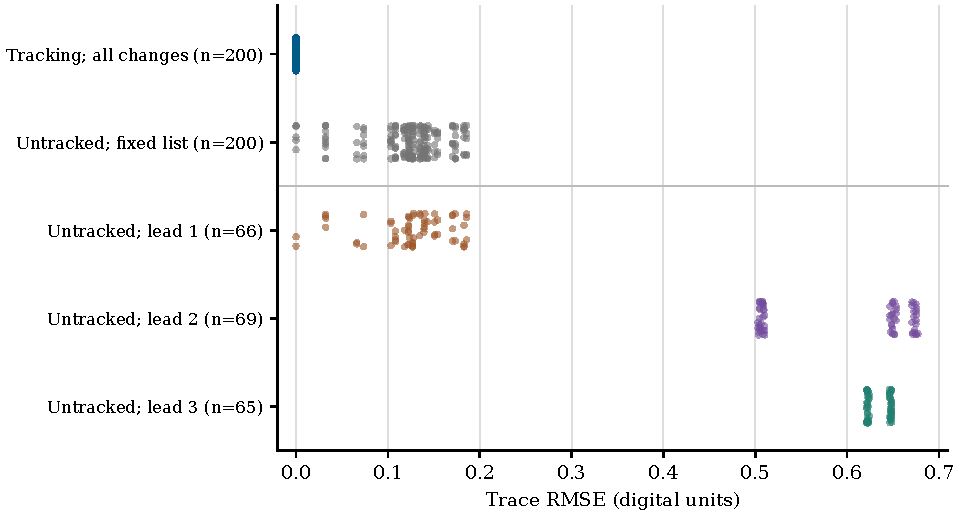
\includegraphics[width=\linewidth]{figures/tracking.pdf}
\caption{Trace errors for the fixed-geometry diagnostic. The lower three rows split the fully permuted untracked trials by leading rectangle: IDs 1, 2, and 3 have perimeters 220, 150, and 90 pixels. Each marker represents one trial; vertical offsets separate overlapping markers and have no quantitative meaning. The two higher-error ranges overlap. These are software checks, not video-quality or analog measurements.}
\label{fig:tracking}
\end{figure}

The untracked errors depend strongly on which contour leads the supplied list. The 66 trials retaining the longest rectangle first have RMSE from 0 to 0.186; the 69 trials leading with the second rectangle have 0.503--0.677; and the 65 leading with the third have 0.621--0.649. The latter two ranges overlap, while neither overlaps the low-error range. The pooled mean, 0.453, falls in the gap between the low- and high-error ranges. Although a valid descriptive mean for the chosen perturbation distribution, it conceals this structure; counts and conditional ranges better expose the observed behavior.

The mechanism follows from \code{order\_contours}: it keeps the first supplied contour and its starting vertex, then chooses and rotates subsequent contours to start at the vertex nearest the preceding start/end point. Changing the leading contour therefore changes scan order and phase. With the original list order fixed, the leading contour's starting vertex and all traversal directions remain variable, while greedy rotation removes some starting-vertex variation from later contours. This accounts for the lower errors in the fixed-order condition.

The fully permuted experiment intentionally bypasses edge extraction to isolate scan construction. Because extraction normally sorts by perimeter, arbitrary permutations of these unequal rectangles are a stronger stress condition than repeatedly extracting the same noiseless image. Perimeter rankings can change with geometry or detection in actual video, but that behavior is not measured here. Two fully permuted baseline trials reproduced the reference waveform. The results indicate waveform sensitivity under the constructed perturbations, not an equivalent loss of depicted geometry: different traversals can draw the same outlines. No population confidence interval or general perceptual improvement is inferred from this diagnostic.

\subsection{Frame-clock verification}
For each of four frame rates, 100,000 successive frame sample counts were generated and their cumulative sums compared at every prefix with exact rational target time. Table~\ref{tab:timing} gives all observed per-frame counts and the maximum absolute discrepancy. The error was at most 0.5 sample, equivalent to approximately $11.34~\mu$s at 44.1~kHz; the final discrepancy was zero for each tested sequence. These results concern duration allocation; the separate 25~frames/s PCM test verifies the revised scan-phase behavior.

\begin{table}[t]
\centering\small
\caption{Frame-clock checks at 44,100 stereo samples/s. Each row covers 100,000 frames.}
\label{tab:timing}
\begin{tabular}{@{}lrrr@{}}
\toprule
Frame rate (frames/s) & Samples per frame & Total samples & Max. error (samples)\\\midrule
24 & 1837 or 1838 & 183,750,000 & 0.5\\
25 & 1764 & 176,400,000 & 0\\
30 & 1470 & 147,000,000 & 0\\
$30000/1001$ & 1471 or 1472 & 147,147,000 & 0.5\\\bottomrule
\end{tabular}
\end{table}

\subsection{Raster-to-trajectory example}
Figure~\ref{fig:raster} shows a generated image containing a filled rectangle, circle, and triangle. Default preprocessing resizes it from $320\times240$ to $480\times360$ pixels. The final binary map contains 1,376 nonzero pixels and yields six retained contours, illustrating that three objects need not produce three scan paths. The resulting 735-sample scan allocates 729 samples to contours and six to transitions. The contour allocations are $(147,145,124,122,96,95)$ samples, and the largest absolute coordinate is approximately 0.67975. The plotted geometry uses the produced samples; it does not simulate DAC filtering, phosphor persistence, or beam intensity.

\begin{figure}[htbp]
\centering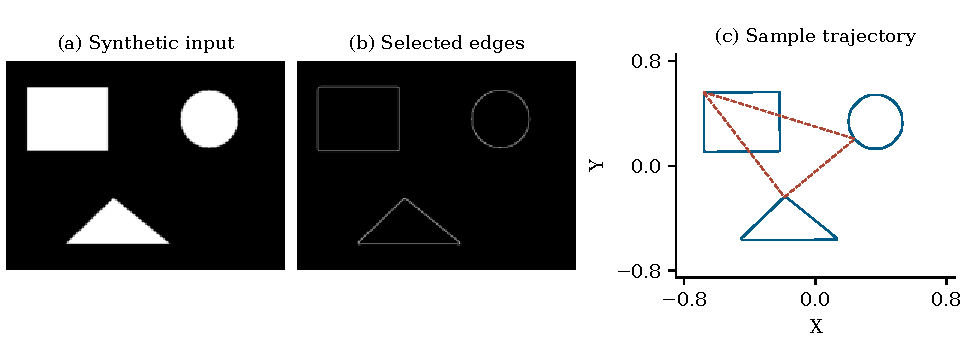
\includegraphics[width=\linewidth]{figures/pipeline_example.pdf}
\caption{A synthetic raster example processed with the default parameters. Solid blue lines connect contour samples; dashed red lines identify inter-contour transitions. Both types of motion are present in the actual two-channel command. The drawing is an ideal sample-space visualization, not an oscilloscope photograph.}
\label{fig:raster}
\end{figure}
\FloatBarrier

\subsection{Fixed-image processing benchmark}
A separate interleaved comparison measures the four processing stages on a $640\times480$ synthetic image containing ten nonoverlapping filled rectangles, resized to width 480. Extraction retains 20 contours. The baseline and revised modules have separate tracker states; each receives ten warm-up iterations, followed by 100 measured iterations. Execution order alternates each iteration. OpenCV is set to one thread, and wall-clock intervals use \code{perf\_counter\_ns}. The machine reports an Intel64 Family~6 Model~158 Stepping~13 processor. The revised arm reuses CLAHE; the baseline creates it per frame.

\begin{table}[htbp]
\centering\small
\caption{Mean stage time in milliseconds for one fixed-image processing run (100 measurements per arm). The total interval excludes capture, decoding, export, preview, pacing, and audio callbacks.}
\label{tab:performance}
\begin{tabular}{@{}lrr@{}}
\toprule
Stage & Public baseline & Revised implementation\\\midrule
Edge preprocessing & 4.75 & 4.78\\
Contour extraction & 0.52 & 0.53\\
Tracking update & 17.10 & 11.39\\
Scan construction & 4.53 & 2.39\\\midrule
Total & 26.89 & 19.07\\\bottomrule
\end{tabular}
\end{table}

Table~\ref{tab:performance} shows a 29.1\% decrease in mean total processing time. Median totals are 26.35 and 18.44~ms; interquartile ranges are 25.69--27.42 and 18.05--19.21~ms for baseline and revised arms, respectively. All 110 paired scan arrays, including warm-up, match exactly. Separate instrumentation counts 60 resampling calls inside tracking and 20 inside scan construction per fully matched frame. The largest absolute saving is consequently in tracking. The small preprocessing difference does not establish a benefit from CLAHE reuse, and this combined comparison does not isolate each edit's contribution. Repetitions of a single static scene and machine support a local cost comparison, not a portable speedup or sustained video-frame-rate claim.

\FloatBarrier

\section{Engineering limits and directions for evaluation}
\subsection{Bandwidth and the physical display}
A digital coordinate stream defines commands to a physical reconstruction chain. A useful linear approximation is
\begin{equation}
 \widetilde x(t)=g_x\sum_n x[n]h_x(t-n/f_s)+b_x,\qquad
 \widetilde y(t)=g_y\sum_n y[n]h_y(t-n/f_s)+b_y,
 \label{eq:hardware}
\end{equation}
where $h_x,h_y$ combine reconstruction and deflection responses, $g_x,g_y$ are gains, and $b_x,b_y$ represent offsets. These parameters are not measured or estimated by video2xy. Unequal gain or phase response distorts shape; AC coupling alters slowly varying components and offsets. Short digital jumps and sharp polygon corners require frequency content that a practical audio interface or display may attenuate.

Sampling theory permits faithful reconstruction only under appropriate bandwidth assumptions~\cite{shannon}. A 44.1~kHz sample rate places the Nyquist frequency at 22.05~kHz, but does not establish that the whole output chain has that usable bandwidth, nor that the constructed polygonal scan is band-limited. The implementation performs no explicit bandwidth-constrained trajectory optimization or output smoothing. Increasing $f_s$ supplies more samples at fixed retrace rate; increasing $f_r$ at fixed $f_s$ reduces the available points per drawing. Neither adjustment alone guarantees improved appearance.

Brightness is also outside the digital model. Approximately uniform arc-length sampling controls dwell along a given contour, but minimum allocations, duplicate endpoints, transition speed, phosphor response, and repeated boundaries affect exposure. A stationary zero-output command is not an intensity-off command. A calibrated hardware evaluation should therefore measure contour and connector brightness separately, alongside gain, coupling, settling, and frequency response. The repository preview overlays polygons on the source image and displays the edge map; it is not a reconstruction of the sampled analog trace.

\subsection{Temporal and computational limits}\label{sec:temporal-limits}
The tracker can confuse nearby contours with similar size and perimeter. Its gates also reject sufficiently large translations or changes in size. Splits, merges, and detection flicker have no explicit model; absence removes a track immediately. Furthermore, contour sample allocations can change when other contours appear or disappear, altering scan timing even when an individual contour retains its identity and starting point. Thus the exact invariance demonstrated in Section~\ref{sec:verification} has a deliberately restricted scope.

Processing resolution, edge density, retained vertex count, and contour count determine cost. The default contour cap bounds association work but does not make it inexpensive. Alignment resamples the previous, forward, and reversed polygons separately, giving three 33-point resampling calls per match. Scan construction adds one call per drawn contour. A frame with 20 matched and drawn contours therefore makes 60 calls inside tracking and 20 inside scan construction; a supplementary fixed-image check confirmed these counts. Resampling optimization can consequently affect both stages. The callback architecture separates scan repetition from camera stalls; this is an architectural property, not a measured throughput result. The fixed-image timings in Table~\ref{tab:performance} cover processing kernels only. No sustained frames-per-second benchmark, end-to-end latency distribution, natural-video dataset, hardware comparison, or listener study is reported here.

The revised parameter checks remove the reproduced clock, allocation, and late-Sobel-validation failures, but do not make the processing chain a general numerical geometry library. Floating-point closure residuals remain, and very large valid-looking budgets may exceed available memory. The unused nearest-vertex helper has been removed. Reversing a forward 33-sample array in place of resampling the reversed polygon was not adopted: finite-precision results can differ, so all three orientation resamplings remain explicit.

\subsection{Evaluation and extensions}
The next evaluation should use fixed, shareable clips covering line art, textured scenes, camera noise, crossings, occlusions, and scene cuts, with all parameters and dependency versions recorded. A tracking ablation should distinguish geometric fidelity from waveform stability and record contour identity changes, jump distance, sample-to-sample motion, processing latency, and audio underflows. Hardware captures would allow edge-location error and connector brightness to be measured against the intended trajectory after calibration.

Further engineering extensions include calibrated bandwidth-aware interpolation, a joint association method for ambiguous contours, and curvature-aware sample allocation. A third output channel could support true intensity blanking on compatible equipment. Each extension changes the tradeoff between complexity, timing, and display fidelity and requires further evaluation.

\section{Conclusion}
video2xy provides an inspectable implementation of raster-video conversion to stereo XY scan commands. The revision preserves tested contour-representation behavior while vectorizing resampling, enforcing feasible scan budgets and supported frame rates, and carrying scan phase across exported video frames. WAV and live output now share boundary-adoption logic while retaining different timing sources. Executed regressions and baseline comparisons establish the stated finite numerical and scheduling properties, and a fixed-image benchmark measures reduced processing cost. Analog fidelity, general temporal robustness, and sustained hardware performance remain subjects for further evaluation.

\section{Code and reproducibility}\label{sec:repro}
The public project is available at \url{https://github.com/peterschwendner/video2xy}. Its baseline revision is
\begin{center}\small\code{6a7d1dd8be7622966f6e4d7e5f2dfbdec1001af6}.\end{center}
The implementation tested in this revision of the paper is local commit
\begin{center}\small\code{cc7fe7a82c60362b43f500489821624e65326bf2}.\end{center}
The supplied source package and Git bundle preserve that update; it had not been pushed to the public repository when these checks were recorded. The bibliography's repository citation identifies the public baseline, not an asserted online location for the local commit. No software licence was added in this revision; licence selection remains with the author.

The update adds installable project metadata, a command-line entry point, runtime dependency ranges, pinned verification dependencies, and a GitHub Actions configuration for Ubuntu and Windows with Python~3.12 and 3.13. Local Python~3.12 verification and wheel construction were executed; hosted CI runs and the other runtime/platform combinations were not verified here.

The accompanying manuscript package includes executable experiment and comparison scripts, the original comparison module, raw CSV and JSON results, test output, source hashes, and generated figures. Leading-contour identifiers support the conditional representation analysis. Reproduction instructions distinguish running the code, reproducing experiments, and compiling the paper. All experimental images and geometry are generated procedurally; no third-party video dataset is used. The measured dependency versions document this run rather than the full supported compatibility range.

\section*{Disclosure of AI assistance}
The author reports using OpenAI Codex in developing video2xy. OpenAI Codex implemented the revised code and regression tests described here and assisted in preparing this manuscript, including source-code inspection, literature discovery, mathematical exposition, writing and executing the supplementary software checks, figure generation, and drafting and editing the text. Reported numerical results were obtained by executing the identified code and are not language-model estimates. The inspected repository does not identify the model version or complete prompt history used during the original development. AI systems are not listed as authors; responsibility for the accuracy, attribution, interpretation, and final approval of the manuscript rests with the human author.

Two user-supplied reviews attributed to Claude informed the code changes and manuscript revisions. Their numerical suggestions and implementation claims were checked against preserved source and executed comparisons. The implemented resampler uses left insertion, and the clock fix rejects unsupported rates; these differ from the reviews' proposed patches for reasons established by boundary cases. Timings reported here were measured locally and do not reuse unverified timing claims from the reviews.

\begingroup
\small\raggedright
\bibliographystyle{IEEEtran}
\bibliography{references}
\endgroup
\end{document}
